\clearpage
%\begin{savequote}[8cm]
%\textlatin{Neque porro quisquam est qui dolorem ipsum quia dolor sit amet, consectetur, adipisci velit...}
%
%There is no one who loves pain itself, who seeks after it and wants to have it, simply because it is pain...
%  \qauthor{--- Cicero's \textit{de Finibus Bonorum et Malorum}}
%\end{savequote}

\chapter{\label{ch:5-mcefficiencies}MC samples and efficiencies} 

\minitoc

\section{MC generation}

Various MC samples were generated for signal and background studies. Both magnet polarities were generated, and both 2011 and 2012 samples were generated with \pythia 8 and Sim08. Also, 2015 and 2016 samples were generated using \pythia 8 and Sim09b. All MC was generated with all daughters in \lhcb acceptance. Signal MC is generated with the \Kstarm forced to \KS$\pim$.

\section{MC efficiencies}
\label{sec:mc:efficiencies}

The signal efficiency of the stripping, trigger and offline selection extracted from MC are listed in Tables \ref{MCeffrun1} and \ref{MCeffrun2} along with the sample size of signal MC decays. These values have been calculated from combined 2011 and 2012 samples and separately from 2015 samples. It can be seen that the LL selection efficiency drops in Run 2, this is thought to be due to the \KS momentum being slightly higher in Run 2 giving fewer \KS mesons decay within the \velo. PID efficiencies have not been included in these calculations; they are extracted from the {\tt PIDCalib} package~\cite{PIDCalib} and are detailed in Section \ref{sec:mc:pid}.

These MC efficiencies are implemented in the analysis as corrections in the \CP fit. For the GLW modes, the ratio $\mathcal{R_{CP}}$, defined in Equation \ref{effcorrectionglw}, multiplies the raw value of $N(KK)/N(K\pi)$ such that the fit results returned, $R_{KK}$ and $R_{\pi\pi}$, are efficiency corrected. The PID efficiencies in Equation \ref{effcorrectionglw} are discussed in Section \ref{sec:mc:pid}.

\begin{equation}
\mathcal{R_{CP}} = \frac{\BR(\decay{\Dz}{\Km\pip})}{\BR(\decay{\Dz}{\Kp\Km})} \times \frac{\epsilon_{sel}(K\pi)}{\epsilon_{sel}(KK)} \times \frac{\epsilon_{pid}(K\pi)}{\epsilon_{pid}(KK)}
\label{effcorrectionglw}
\end{equation}

As the final state in the ADS mode is almost identical to the charge favoured, the selection efficiencies that are common to both are assumed to cancel. There are only two differences between the selection for the ADS mode and the charge favoured mode; the tighter BDT selection for DD candidates and the double misID veto, which is only applied to the ADS mode. Efficiency corrections need to be made for these differences in selection. For the ADS mode, the ratio $\mathcal{R_{ADS}}$, defined in Equation \ref{effcorrectionads}, multiplies the raw value of $N(\pi K)/N(K\pi)$ such that the fit results returned, $R^+$ and $R^-$, are efficiency corrected. This correction includes the ratio of BDT efficiencies, discussed in Section \ref{sec:mc:bdt}, and the veto efficiency, discussed in Section \ref{sec:mc:pid}.

\begin{equation}
\mathcal{R_{ADS}} = \frac{\epsilon_{BDT}(K\pi)}{\epsilon_{BDT}(\pi K)} \times \frac{1}{\epsilon_{veto}(\pi K)}
\label{effcorrectionads}
\end{equation}

For the 4 body mode, efficiency corrections are applied equivalent to those in Equations \ref{effcorrectionglw} adn \ref{effcorrectionads}.

The final fit to the data measures $A_{K\pi}$, $A_{KK}$, $A_{\pi\pi}$, $R_{KK}$, $R_{\pi\pi}$, $R^+$,  $R^-$, $A_{K\pi\pi\pi}$, $A_{\pi\pi\pi\pi}$, $R_{\pi\pi\pi\pi}$, $R^+_{K3\pi}$ and  $R^-_{K3\pi}$, which all have the relevant efficiency corrections applied.

\begin{table}[h]
\centering
\begin{tabular}{ccccc}
\hline
& \multicolumn{2}{c}{Run 1} & \multicolumn{2}{c}{Run 2} \\
Decay mode & $\epsilon_{sel}(\%)$ & $N_{sel}$ & $\epsilon_{sel}(\%)$ & $N_{sel}$ \\
\hline
$B^{\pm} \to [K^{\pm}\pi^{\mp}]_D K^{*\pm}$ & $0.0939 \pm 0.0011$ & 2198 & $0.1266 \pm 0.0011$ & 5105 \\
$B^{\pm} \to [K^{\pm}K^{\mp}]_D K^{*\pm}$ & $0.0919 \pm 0.0011$ & 2129 & $0.1189 \pm 0.0010$ & 4871 \\
$B^{\pm} \to [\pi^{\pm}\pi^{\mp}]_D K^{*\pm}$ & $0.1015 \pm 0.0012$ & 2363 & $0.1292 \pm 0.0011$ & 5281 \\
$B^{\pm} \to [K^{\pm}\pi^{\mp}\pi^{\pm}\pi^{\mp}]_D K^{*\pm}$ & $0.0288 \pm 0.0006$ & 588 & $0.0484 \pm 0.0004$ & 4979 \\
$B^{\pm} \to [\pi^{\pm}\pi^{\mp}\pi^{\pm}\pi^{\mp}]_D K^{*\pm}$ &  &  &  &  \\
\hline
\end{tabular}
\caption{MC signal efficiencies and yields (LL). For two-body, 2M Run 1 events were generated for each mode and 4M Run 2 events were generated for each mode. For four-body, 2M Run 1 events were generated and 10M Run 2 events were generated. {\color{red}$4\pi$ efficiencies will be added when the MC is available}}
\label{MCeffrun1}
\end{table}

\begin{table}[h]
\centering
\begin{tabular}{ccccc}
\hline
& \multicolumn{2}{c}{Run 1} & \multicolumn{2}{c}{Run 2} \\
Decay mode & $\epsilon_{sel}(\%)$ & $N_{sel}$ & $\epsilon_{sel}(\%)$ & $N_{sel}$ \\
\hline
$B^{\pm} \to [K^{\pm}\pi^{\mp}]_D K^{*\pm}$ & $0.2519 \pm 0.0018$ & 5603 & $0.3155 \pm 0.0017$ & 12748 \\
$B^{\pm} \to [K^{\pm}K^{\mp}]_D K^{*\pm}$ & $0.2450 \pm 0.0018$ & 5404 & $0.2923 \pm 0.0016$ & 11966 \\
$B^{\pm} \to [\pi^{\pm}\pi^{\mp}]_D K^{*\pm}$ & $0.2584 \pm 0.0018$ & 5760 & $0.3309 \pm 0.0017$ & 13603 \\
$B^{\pm} \to [K^{\pm}\pi^{\mp}\pi^{\pm}\pi^{\mp}]_D K^{*\pm}$ & $0.0816 \pm 0.0020$ & 1670 & $0.1229 \pm 0.0007$ & 12605 \\
$B^{\pm} \to [\pi^{\pm}\pi^{\mp}\pi^{\pm}\pi^{\mp}]_D K^{*\pm}$ &  &  &  &  \\
\hline
\end{tabular}
\caption{MC signal efficiencies and yields (DD). For two-body, 2M Run 1 events were generated for each mode and 4M Run 2 events were generated for each mode. For four-body, 2M Run 1 events were generated and 10M Run 2 events were generated. {\color{red}$4\pi$ efficiencies will be added when the MC is available}}
\label{MCeffrun2}
\end{table}


\section{Using MC in TMVA training}
\label{sec:mc:tmva}

For $B^{\pm} \to [K^{\pm}\pi^{\mp}]_D K^{*\pm}$, the number of MC events passing the stripping and going on to be used as a signal training sample was found to be low, which resulted in overtraining of the BDT. In order to deal with this problem MC was produced with generator level cuts such that significantly more events pass the stripping, giving a larger signal sample size to be used in training. The following generator level cuts were applied:

\begin{itemize}
\item{Bu $p\ >$ 50 GeV}
\item{Bu $p_T\ >$ 4.5 GeV}
\item{Bu $\tau\ >$ 0.4 ps}
\item{\Dz p $>$ 20 GeV}
\item{\Dz $p_T\ >$ 2 GeV}
\item{$K_s\ p\ >$ 4.5 GeV}
\item{$K_s\ p_T\ >$ 0.45 GeV}
\item{Bach $p\ >$ 5.5 GeV}
\item{Bach $p_T\ > 5.5 GeV$}
\item{$K_s$ daughters $p\ >$ 2 GeV}
\item{\Dz daughters $p\ >$ 1.5 GeV}
\end{itemize}

These generator level cuts remove 89\% of events at generator level while keeping 78\% of LL candidates and 81\% of DD candidates. Not all generator level cuts are looser than those applied to the data in stripping, however the loss in good signal was deemed to be acceptable to be able to increase signal yields in the MC. Due to the \KS plus 3 track final state the reconstruction efficiency of this decay mode is very low.

For $B^{\pm} \to [K^{\pm}\pi^{\mp}\pi^{\pm}\pi^{\mp}]_D K^{*\pm}$ BDT training Run 2 MC was produced. Run 2 MC can currently be produced in mDST format whereas Run 1 MC cannot. Therefore, a large amount of Run 2 MC was generated (10M events) in order to train the 4 body BDT and avoid overtraining. This allows training of the BDT without having to apply cuts to the sample at the generator level.


\section{Comparison of data and MC distributions}
\label{sec:mc:datavsmc}

Signal MC is used in this analysis to provide a training sample for the BDT. Also both signal and background MC samples are used to provide efficiencies for estimating relative yield contributions and shapes for use in the mass fit. Therefore we require the MC to correctly represent the signal. Figures \ref{mcdataagreementLL} and \ref{mcdataagreementDD} show comparisons between $B^{\pm} \to [K^{\pm}\pi^{\mp}]_D K^{*\pm}$ MC and data distributions for the BDT input variables to BDT\_LL and BDT\_DD respectively with Run 1 and Run 2 data combined. Figure \ref{mcdataagreementbdt} shows comparisons between the BDT response using the same samples. The data sample has passed the full selection and sWeights have been applied, and the MC sample has passed the full selection excluding PID cuts. These distributions show reasonable agreement to validate training the BDT using MC to represent the signal.

\begin{figure}[h]
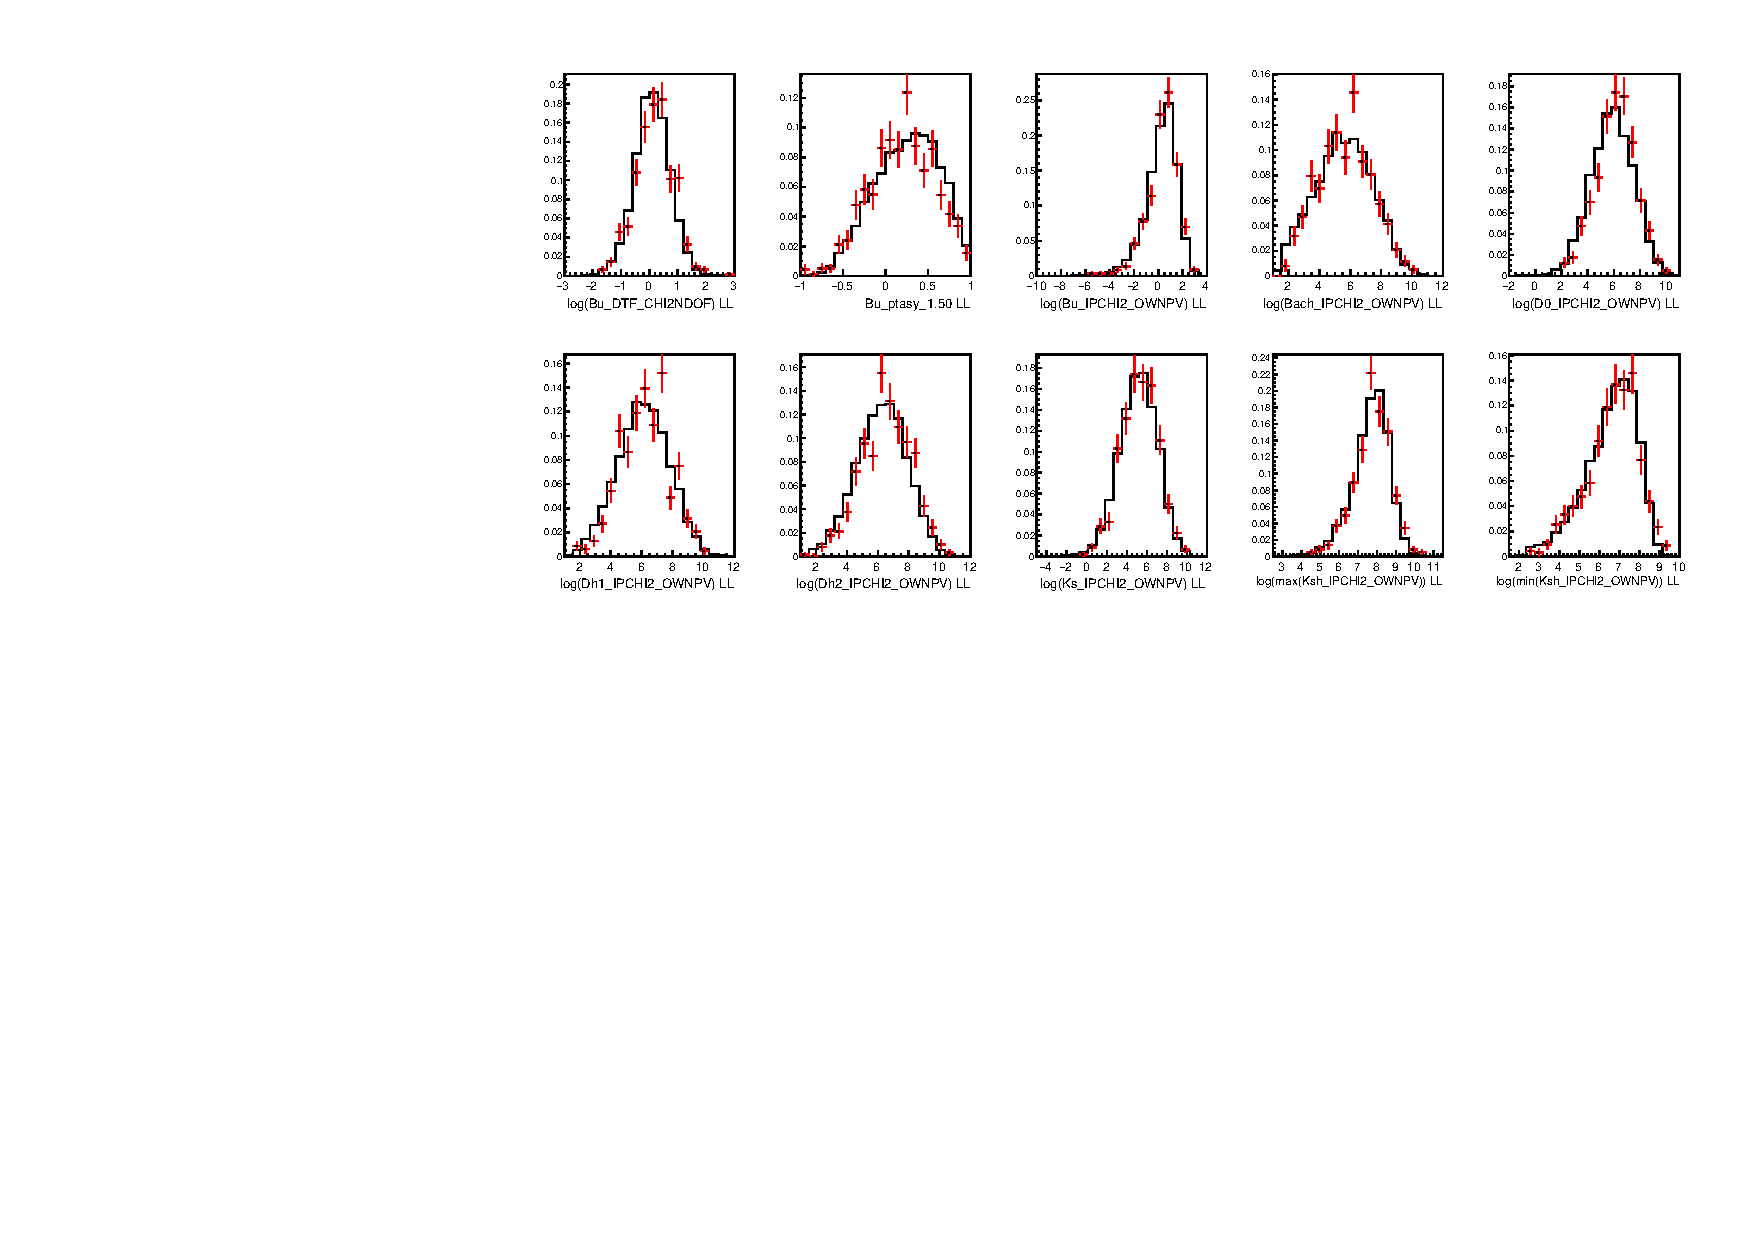
\includegraphics[width=\linewidth]{figures/compareMC/MCdataAgreement_LL.pdf}
\caption{Plots comparing the $B^{\pm} \to [K^{\pm}\pi^{\mp}]_D K^{*\pm}$ MC and data distributions for the BDT input variables for LL candidates. Both data and MC samples are of Run 1 and Run 2 data combined. MC is black and data is red. The errors from MC are significantly smaller than data.}
\label{mcdataagreementLL}
\end{figure}

\begin{figure}[h]
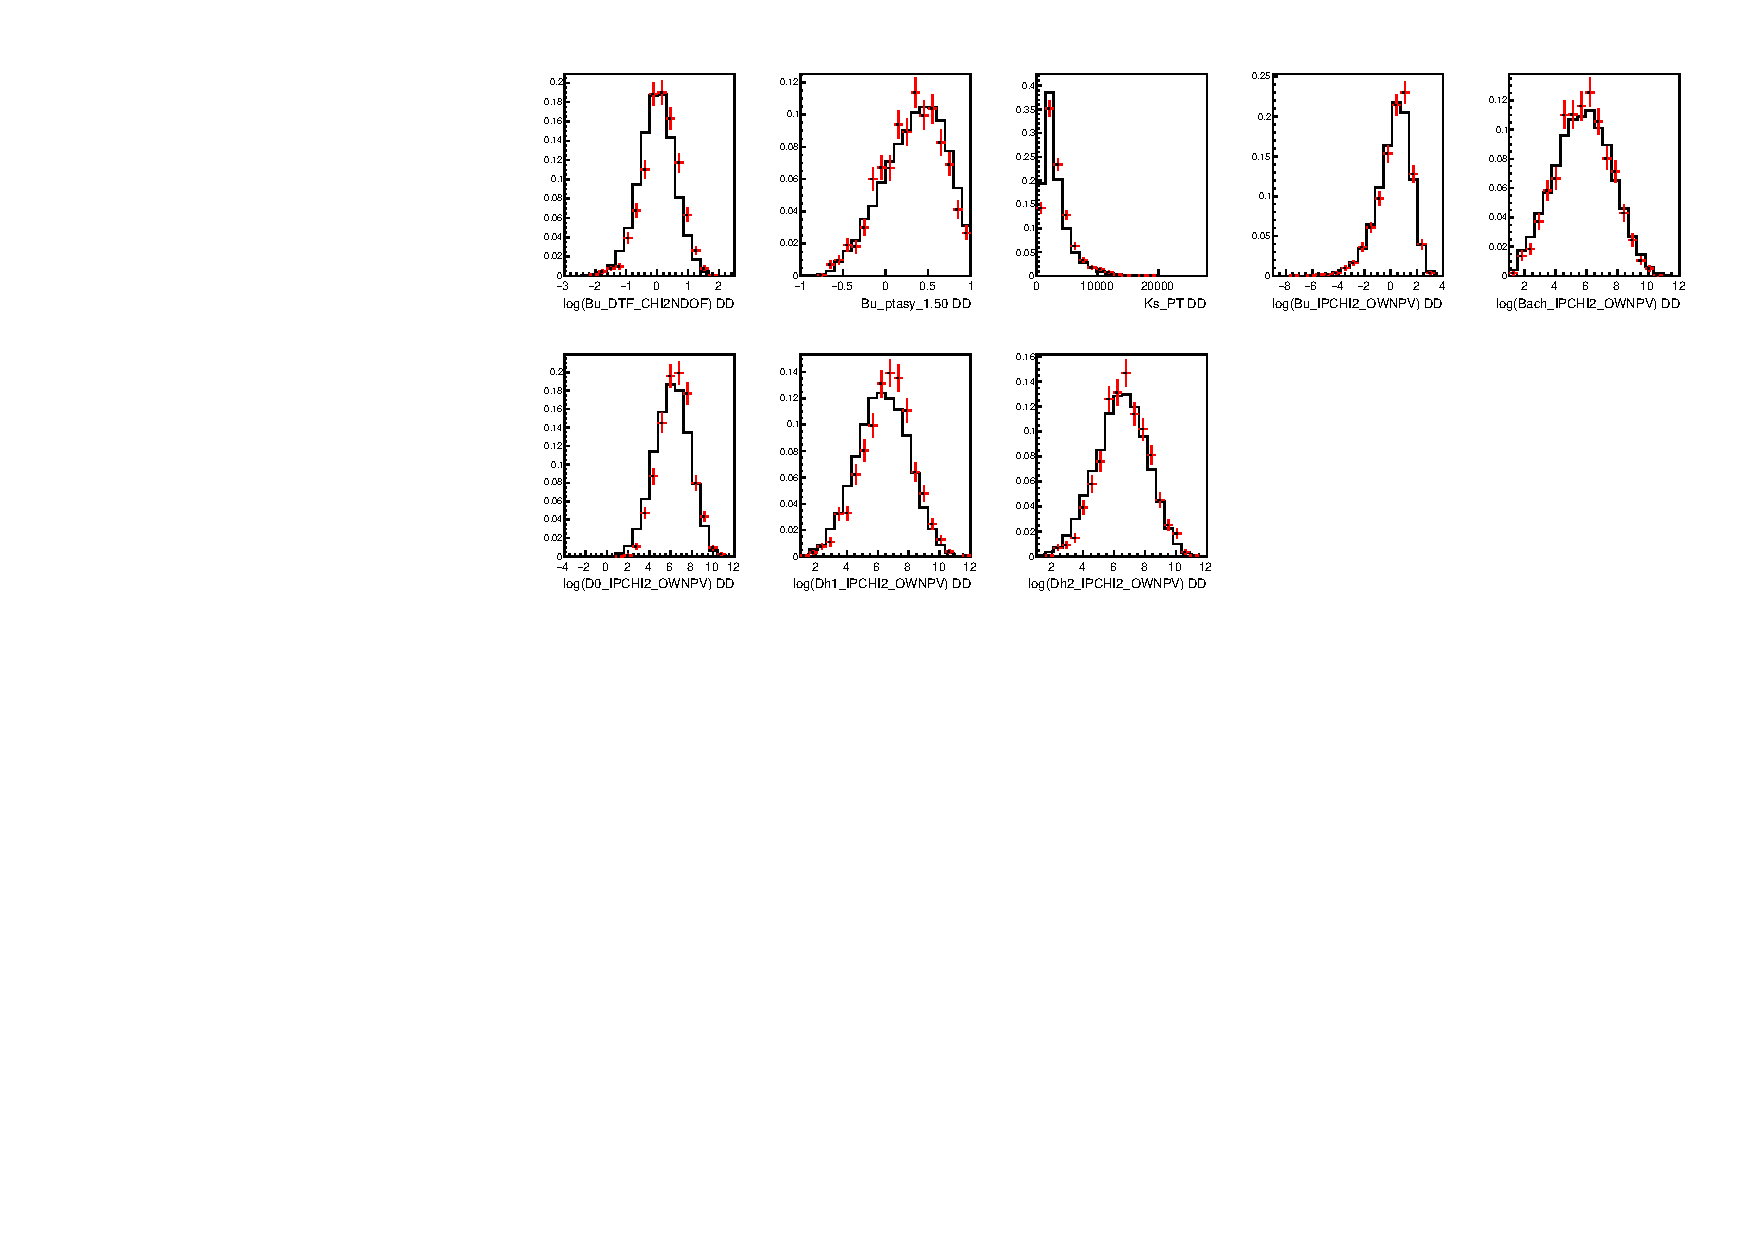
\includegraphics[width=\linewidth]{figures/compareMC/MCdataAgreement_DD.pdf}
\caption{Plots comparing the $B^{\pm} \to [K^{\pm}\pi^{\mp}]_D K^{*\pm}$ MC and data distributions for the BDT input variables for DD candidates. Both data and MC samples are of Run 1 and Run 2 data combined. MC is black and data is red. The errors from MC are significantly smaller than data.}
\label{mcdataagreementDD}
\end{figure}

\begin{figure}[h]
\centering
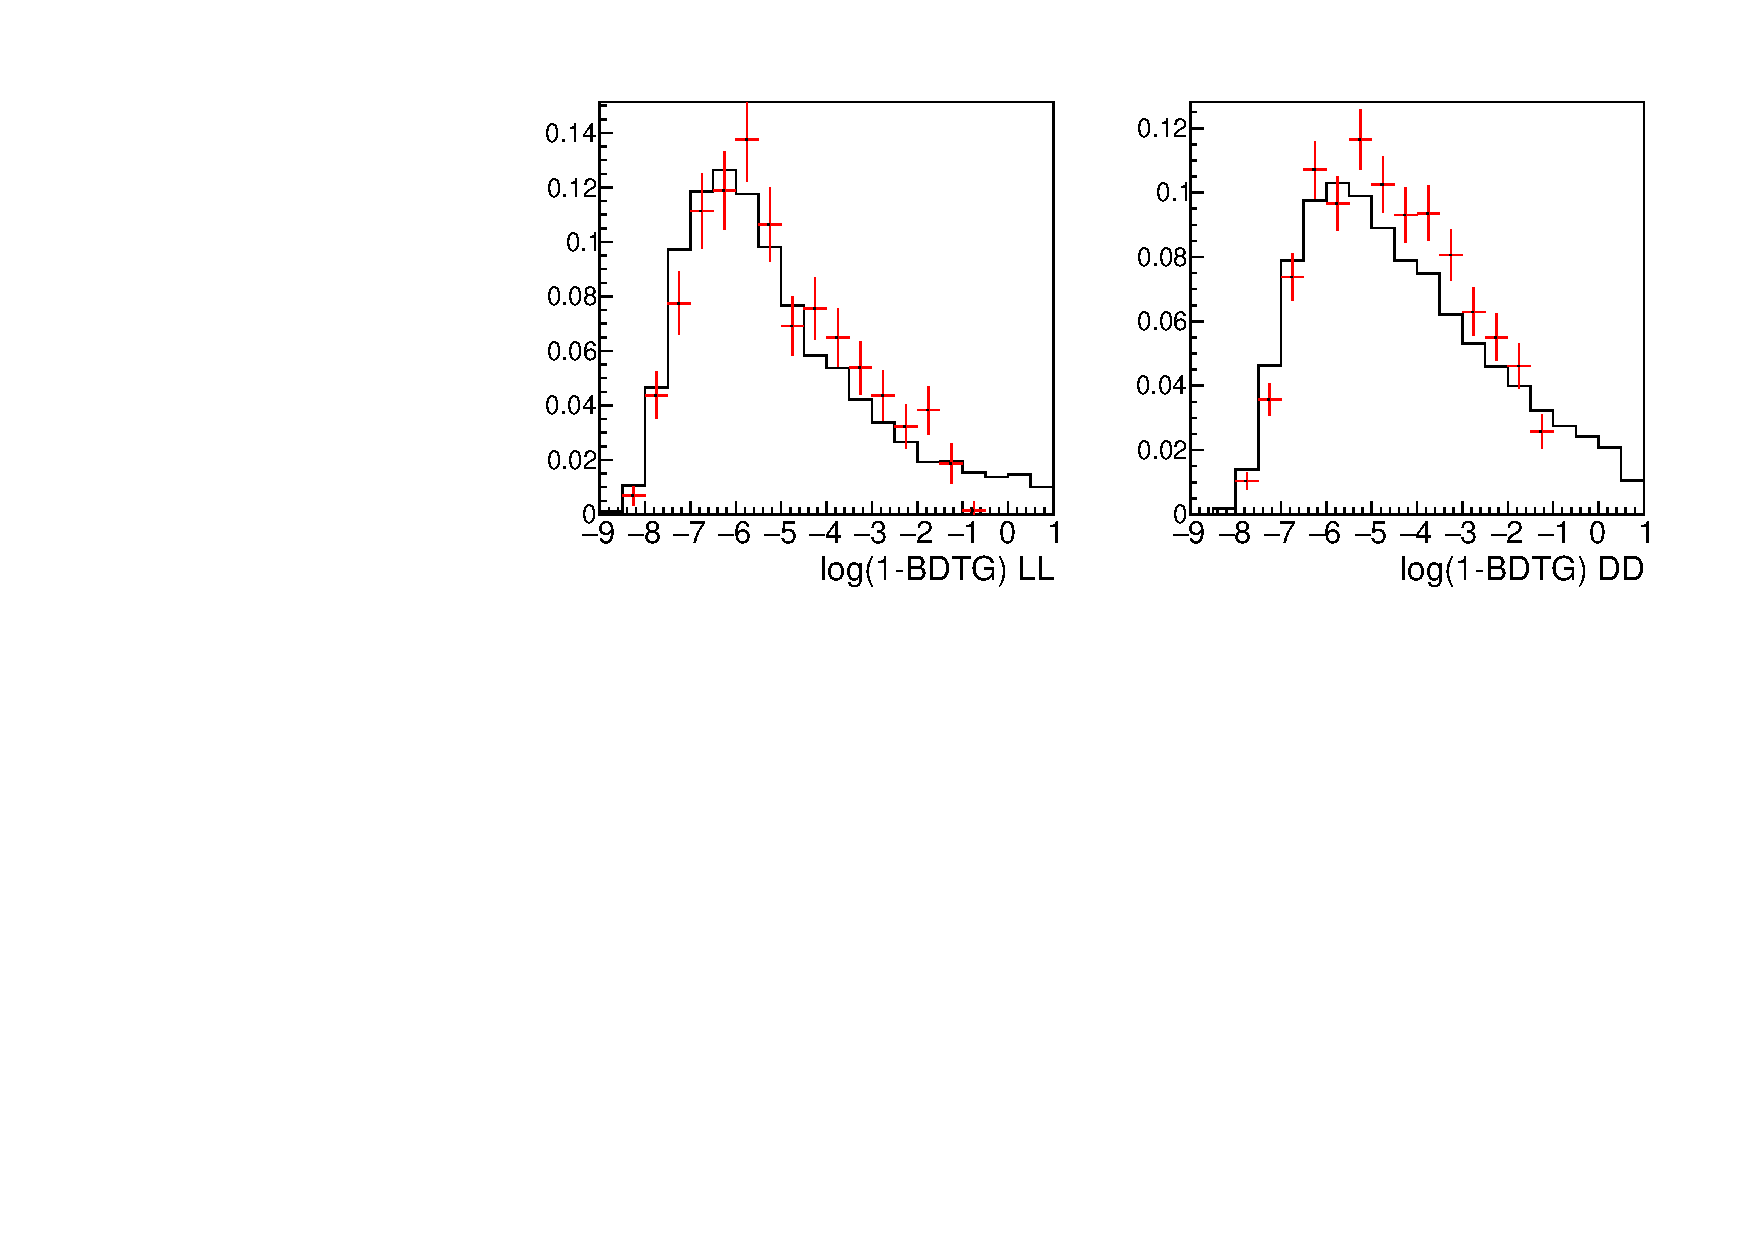
\includegraphics[width=0.7\linewidth]{figures/compareMC/MCdataAgreement_bdtResponse.pdf}
\put(-200,110) {(a)}
\put(-40,110) {(b)}
\caption{Plots comparing the $B^{\pm} \to [K^{\pm}\pi^{\mp}]_D K^{*\pm}$ MC and data distributions for the $log(1 - BDT)$ response for (a) LL candidates, and (b) DD candidates. Both data and MC samples are of Run 1 and Run 2 data combined. MC is black and data is red. The errors from MC are significantly smaller than data.}
\label{mcdataagreementbdt}
\end{figure}

The MC efficiencies will depend on the production kinematics therefore it is important for the data and MC samples to be consistent in kinematic variables of the B candidate. Figure \ref{bkinematics} shows conparison between data and MC for kinematic variables of the B candidate. It can be seen that these distributions are consistent in momentum, transverse momentum and pseudorapidity.

\begin{figure}
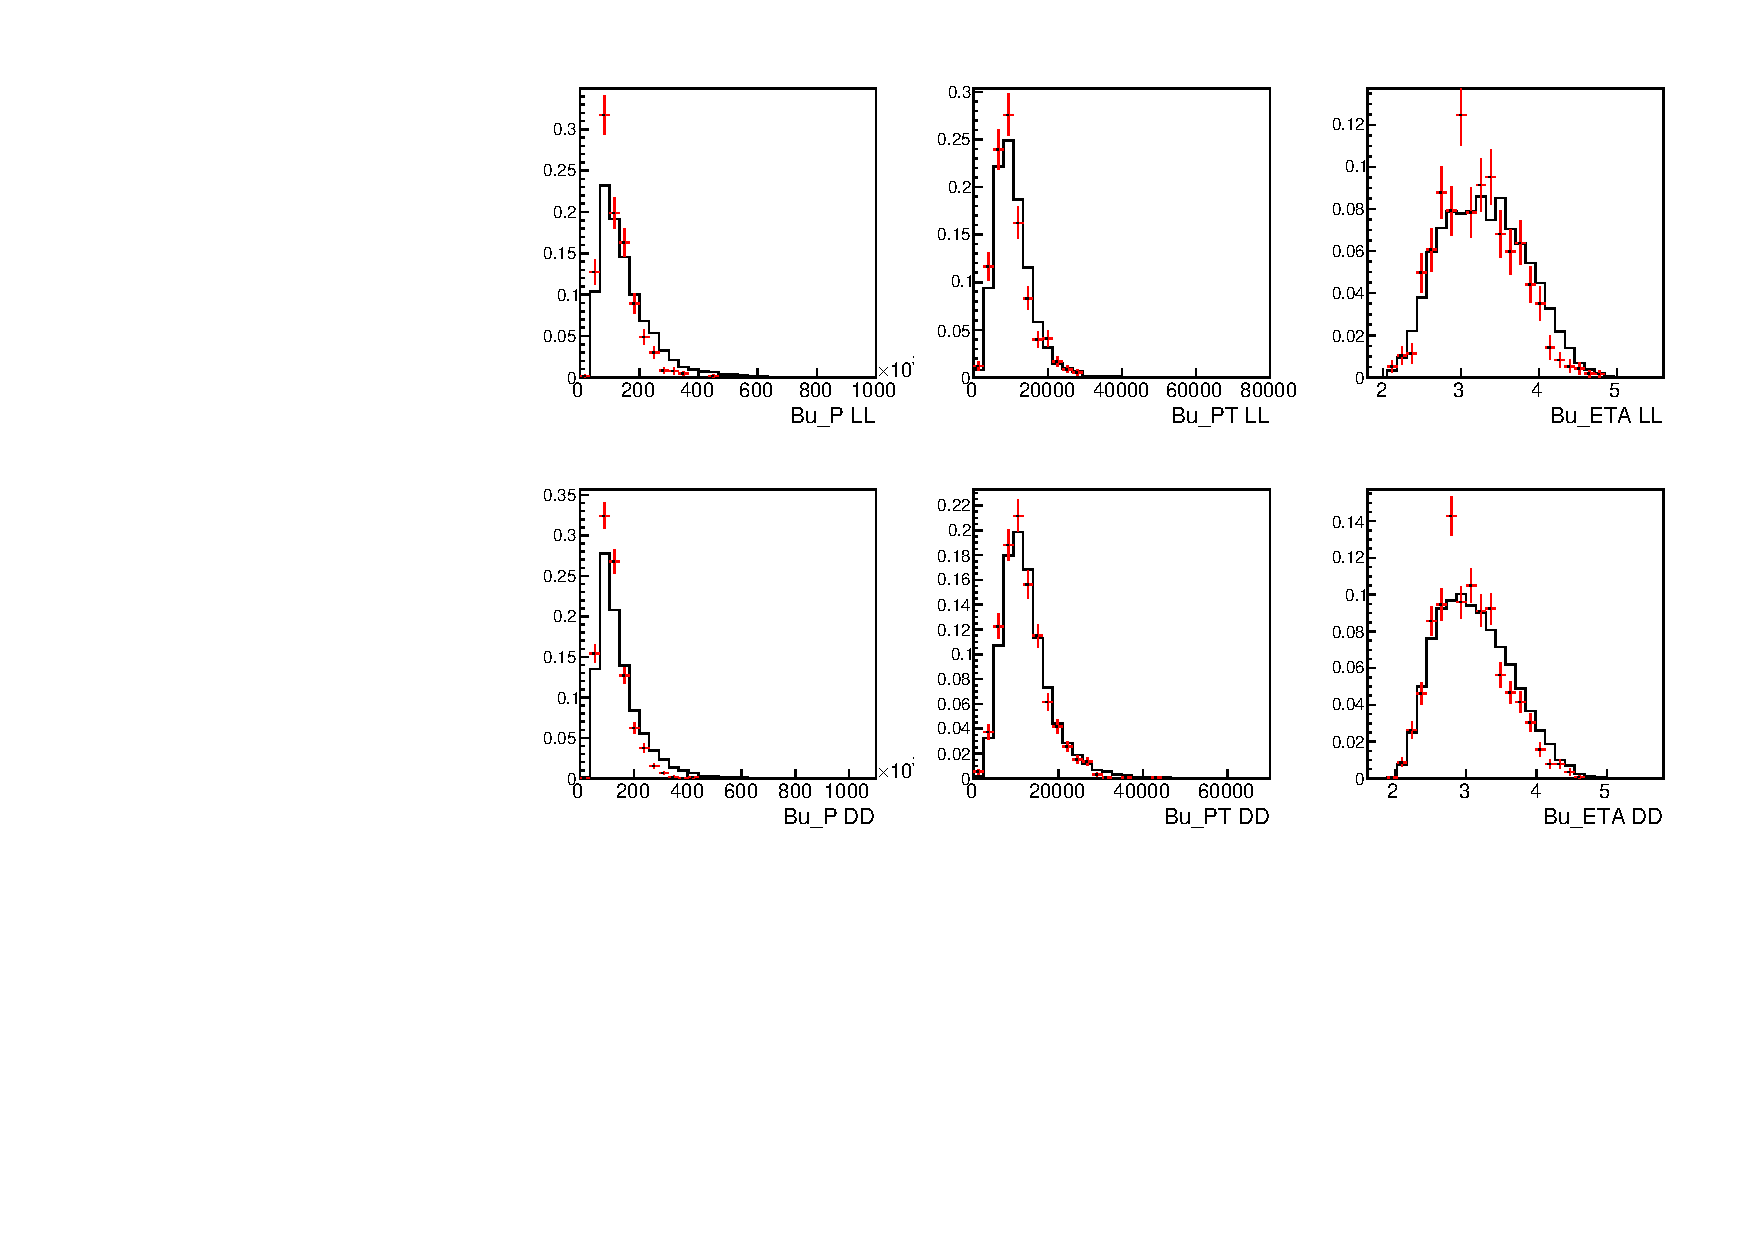
\includegraphics[width=\linewidth]{figures/compareMC/Bkinematics.pdf}
\caption{Plots comparing $B^{\pm} \to [K^{\pm}\pi^{\mp}]_D K^{*\pm}$ MC (black) and data (red) distributions for momentum, $p$, transverse momentum, $p_T$, and pseudorapidity, $\eta$ of the B candidate. Both data and MC samples are of Run 1 and Run 2 data combined. The top row show the distributions for LL candidates and the bottom row are for DD candidates.}
\label{bkinematics}
\end{figure}

\section{Comparison of Run 1 vs Run 2}

This analysis uses MC for training the BDT, fixing shape parameteres in the mass fit and efficiency corrections in the mass fit. As detailed in Section \ref{sec:selection:strippingandtrigger}, data collected in 2011, 2012, 2015 and 2016 are used in this analysis. Several checks were made comparing the Run 1 MC to Run 2 MC.

\subsubsection{BDT training}
\label{sec:mc:bdt}

BDT variable distributions in Run 1 and 2015 MC show minor differences, as shown in Figure \ref{mcrun1vsrun2}. Both samples have had the full selection applied excluding PID cuts. The BDTs were trained on Run 1 MC, as described in Section \ref{sec:selection:bdt}, and then applied to Run 2 MC and the selection efficiencies were found to be similar, as shown in Table \ref{bdtefficiencies2body}. The equivalent results for the 4 body mode are shown in Table \ref{bdtefficiencies4body}.

\begin{figure}
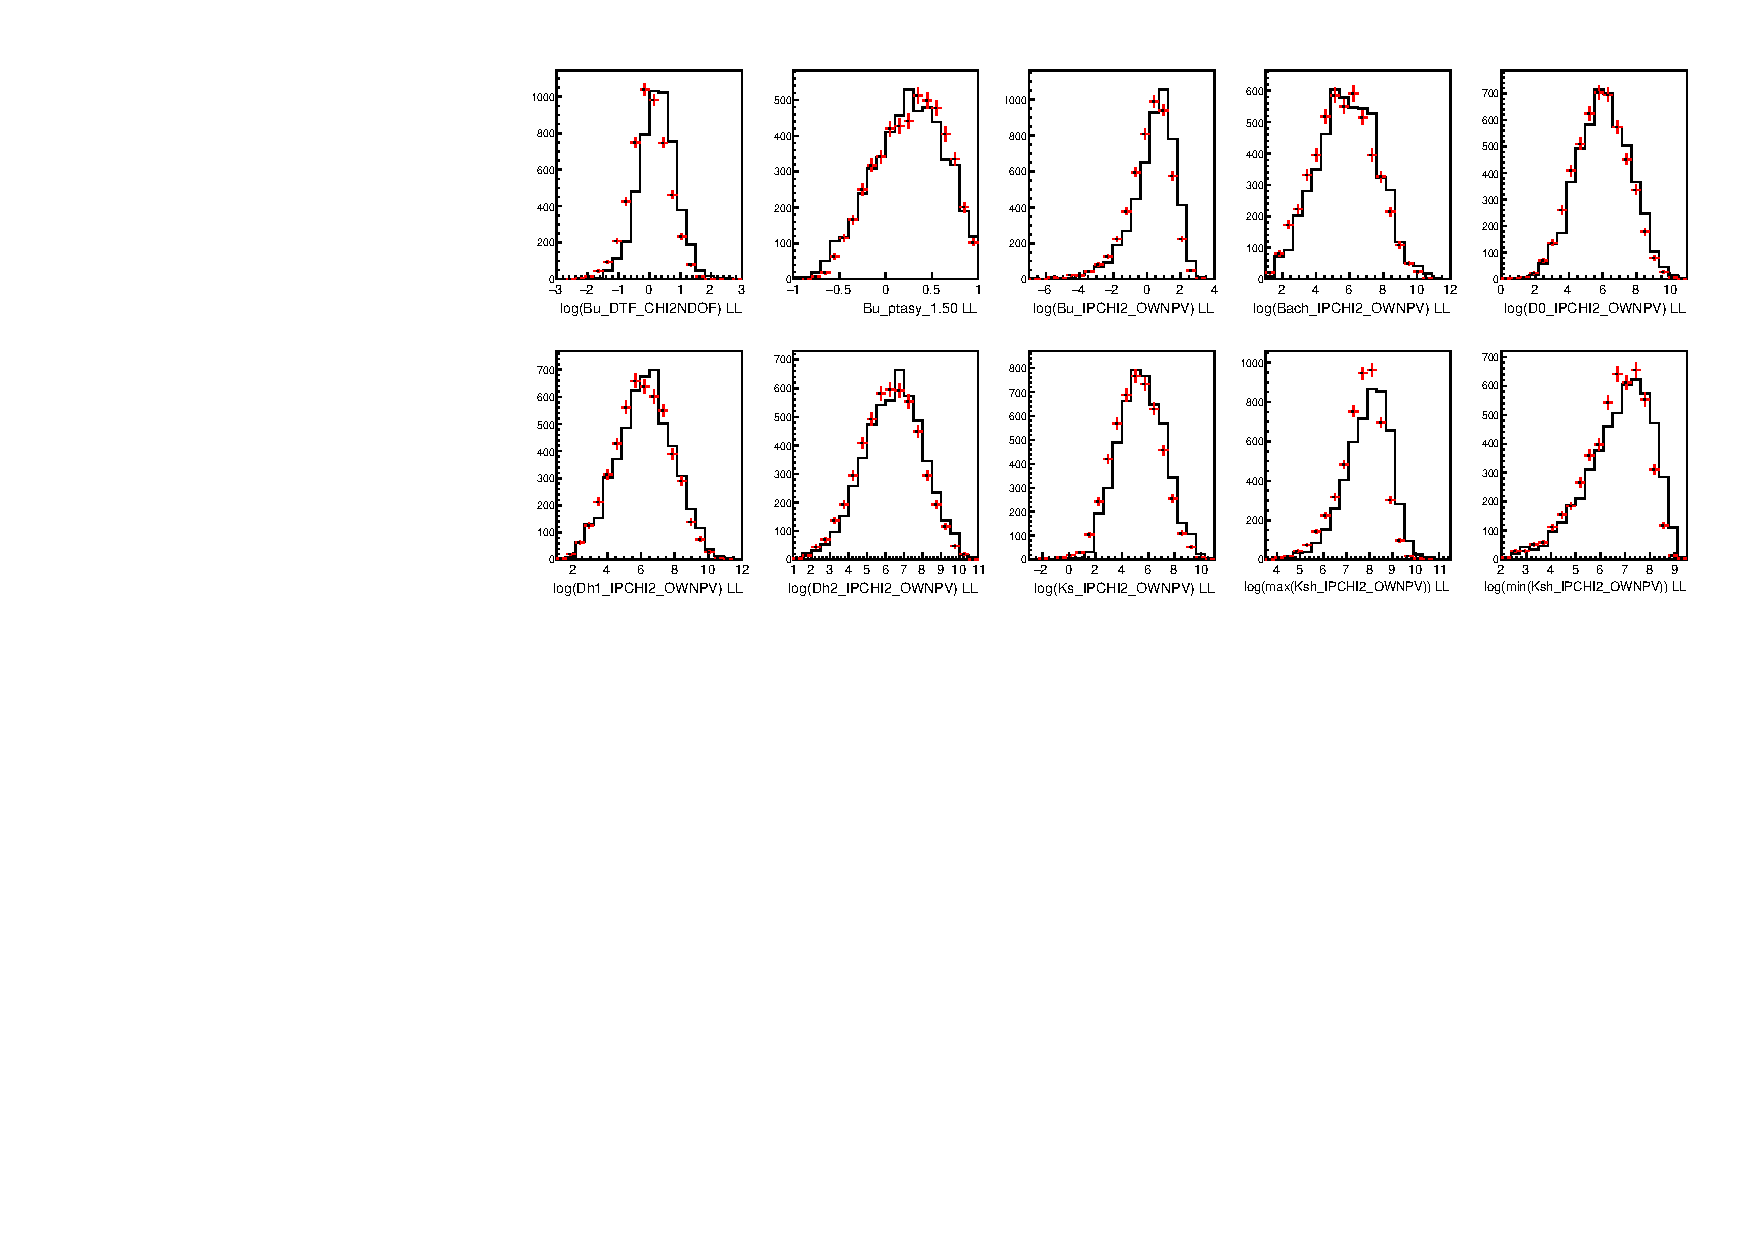
\includegraphics[width=\linewidth]{figures/compareMC/compareMC_run1vsrun2_BDTvariablesLL.pdf}
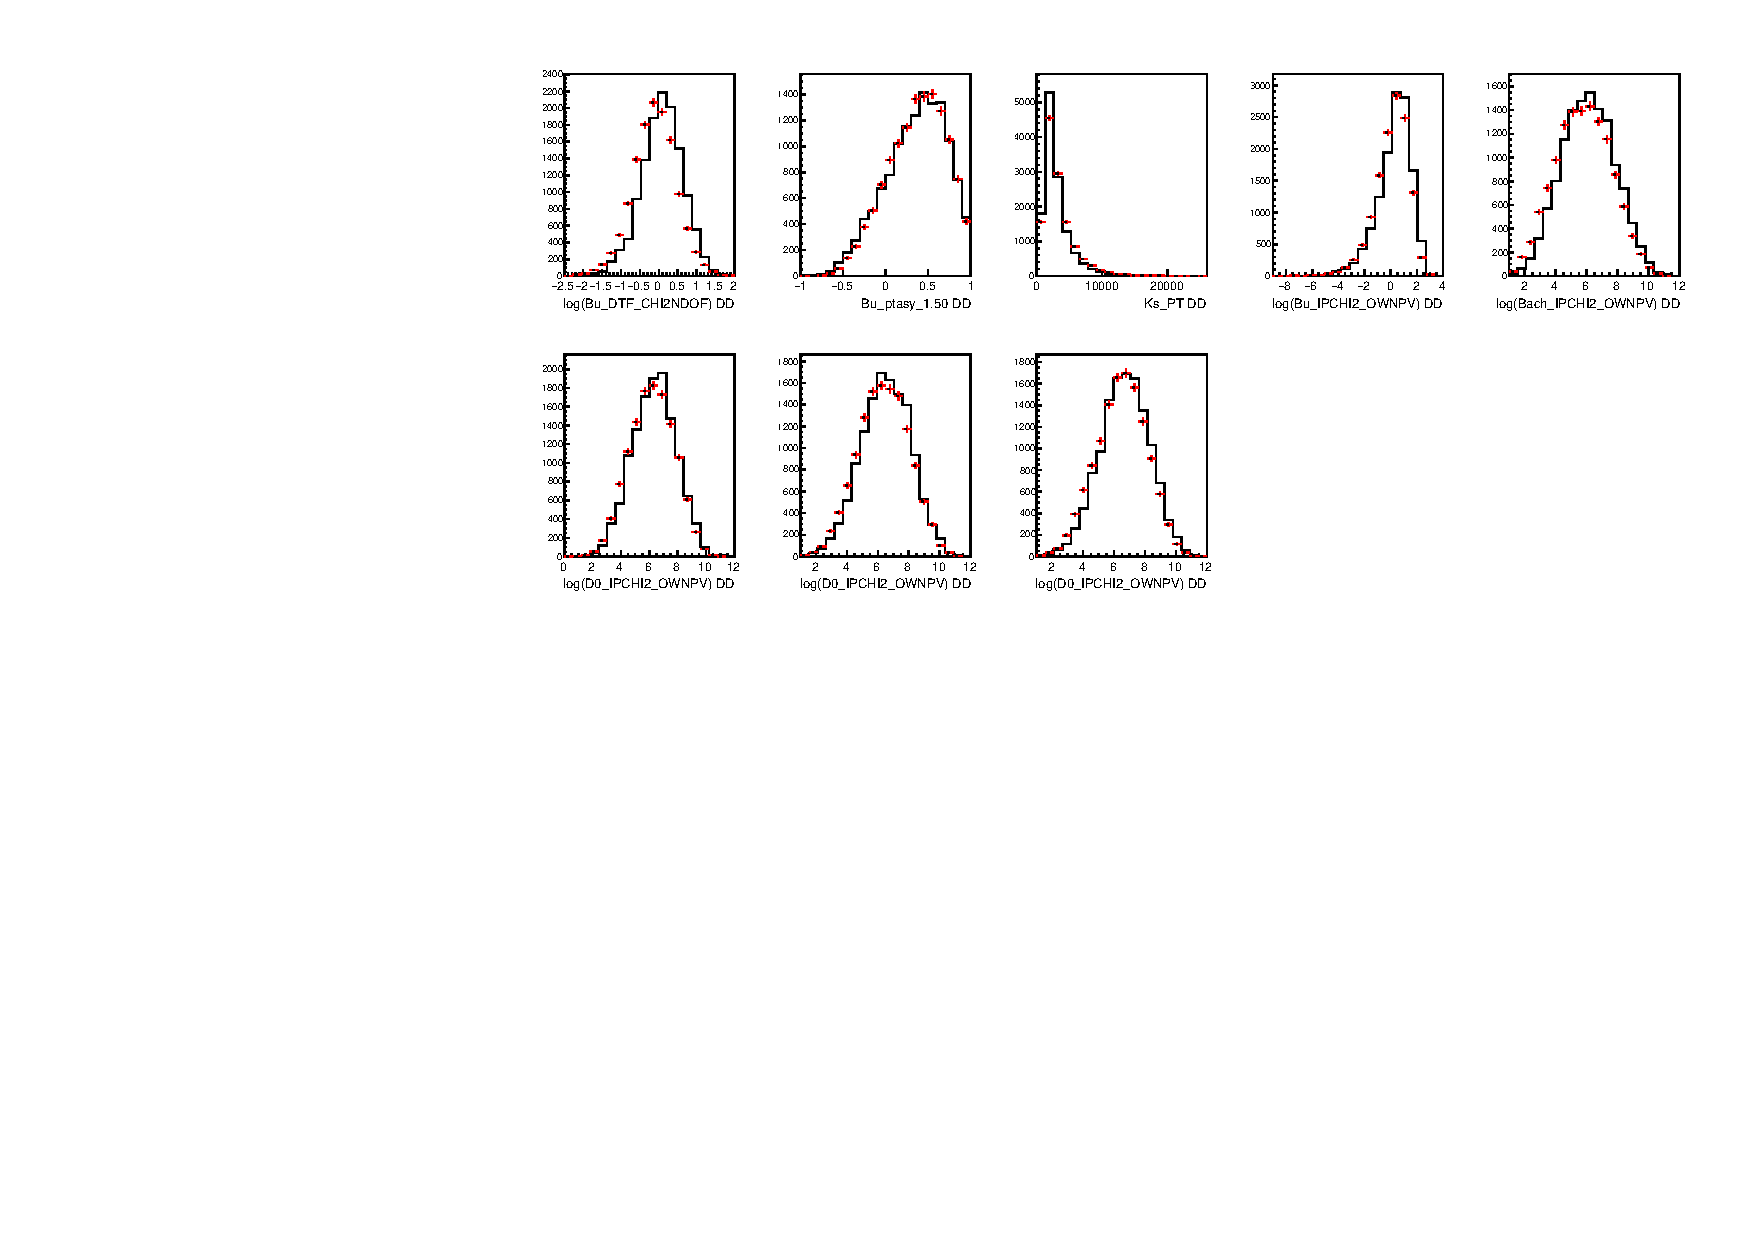
\includegraphics[width=\linewidth]{figures/compareMC/compareMC_run1vsrun2_BDTvariablesDD.pdf}
\caption{Comparison of MC between Run 1 and Run 2. Run 1 MC is black and Run 2 MC is red.}
\label{mcrun1vsrun2}
\end{figure}

\begin{table}[h]
\centering
\begin{tabular}{lll}
\hline
& Run 1 & Run 2 \\
\hline
LL & $0.947 \pm 0.005 $ & $0.949 \pm 0.003$ \\
DD (favoured) & $0.896 \pm 0.004$ & $0.907 \pm 0.002$ \\
DD (ADS) & $0.802 \pm 0.005$ & $0.826 \pm 0.003$ \\
\hline
\end{tabular}
\caption{BDT efficiencies for the $K\pi$ favoured mode when applied to Run 1 and Run 2 MC}
\label{bdtefficiencies2body}
\end{table}

\begin{table}[h]
\centering
\begin{tabular}{lll}
\hline
& Run 1 & Run 2 \\
\hline
LL & $0.938 \pm 0.010 $ & $0.952 \pm 0.003$ \\
DD (favoured) & $0.903 \pm 0.007$ & $0.928 \pm 0.002$ \\
DD (ADS) & $0.838 \pm 0.009$ & $0.870 \pm 0.003$ \\
\hline
\end{tabular}
\caption{BDT efficiencies for the 4 body mode when applied to Run 1 and Run 2 MC}
\label{bdtefficiencies4body}
\end{table}

\subsection{PDF shapes in mass fit}
\label{sec:mc:pdfshapes}

Fits to the refitted B mass distributions have been compared between Run 1 and Run 2 signal MC, the signal PDFs are shown in Figures \ref{signalfitcomparison2body}. These shapes are consistent between Run 1 and Run 2, therefore signal shapes are shared in the simultaneous fit. Further comparisons are made between 2 and 4 body modes. Figure \ref{signalfitcomparisonRun1} compare the signal PDFs obtained from MC between $K\pi$ and $K\pi\pi\pi$ for Run 1 MC. These are noticablely different and so $K\pi$ and $K\pi\pi\pi$ are associated with different signal shapes in the mass fit. The signal shape is discussed in detail in Section \ref{sec:massfit:signal}.

The mean obtained from a fit to signal MC is consistent with that from data, as shown in Table \ref{signalmean}, therefore no shift is applied to the partially reconstructed shapes in MC. Parially reconstructed decays are described in detail in Section \ref{sec:massfit:partreco}. Similar comparisons for partially reconstructed decays are shown in Figure \ref{parterecofits}. These distributions are considered sufficienctly similar to fix the shapes across all years. The parameters for the partially reconstructed shapes are obtained from performing individual fits to Run 1 MC.

\begin{figure}
\centering
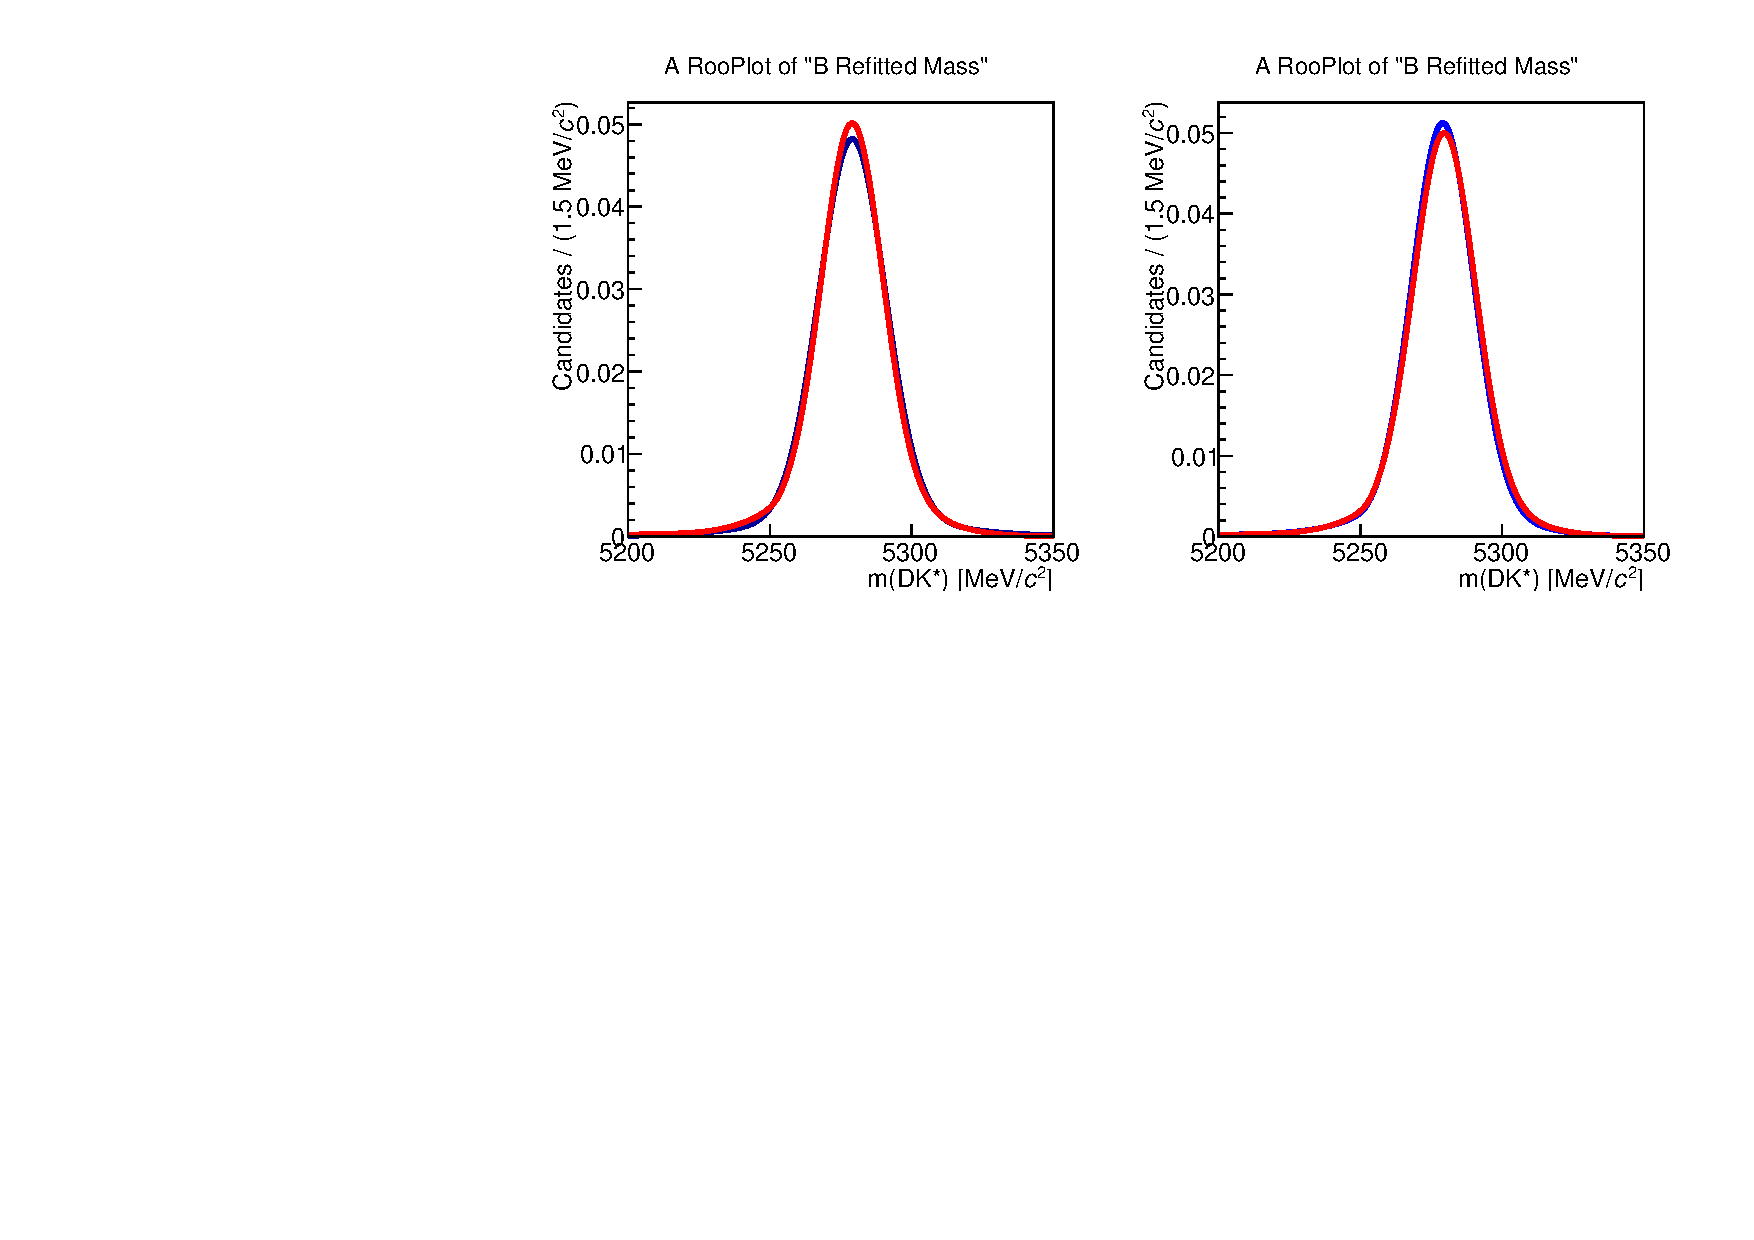
\includegraphics[width=0.7\linewidth]{figures/fitComponents/signalMC_KPi_run1vsrun2.pdf}
\put(-270,110) {(a)}
\put(-120,110) {(b)}
\caption{Comparison of $K\pi$ signal fit functions for Run 1 (blue) and Run 2 MC (red) for (a) LL candidates and (b) DD candidates}
\label{signalfitcomparison2body}
\end{figure}

\begin{figure}
\centering
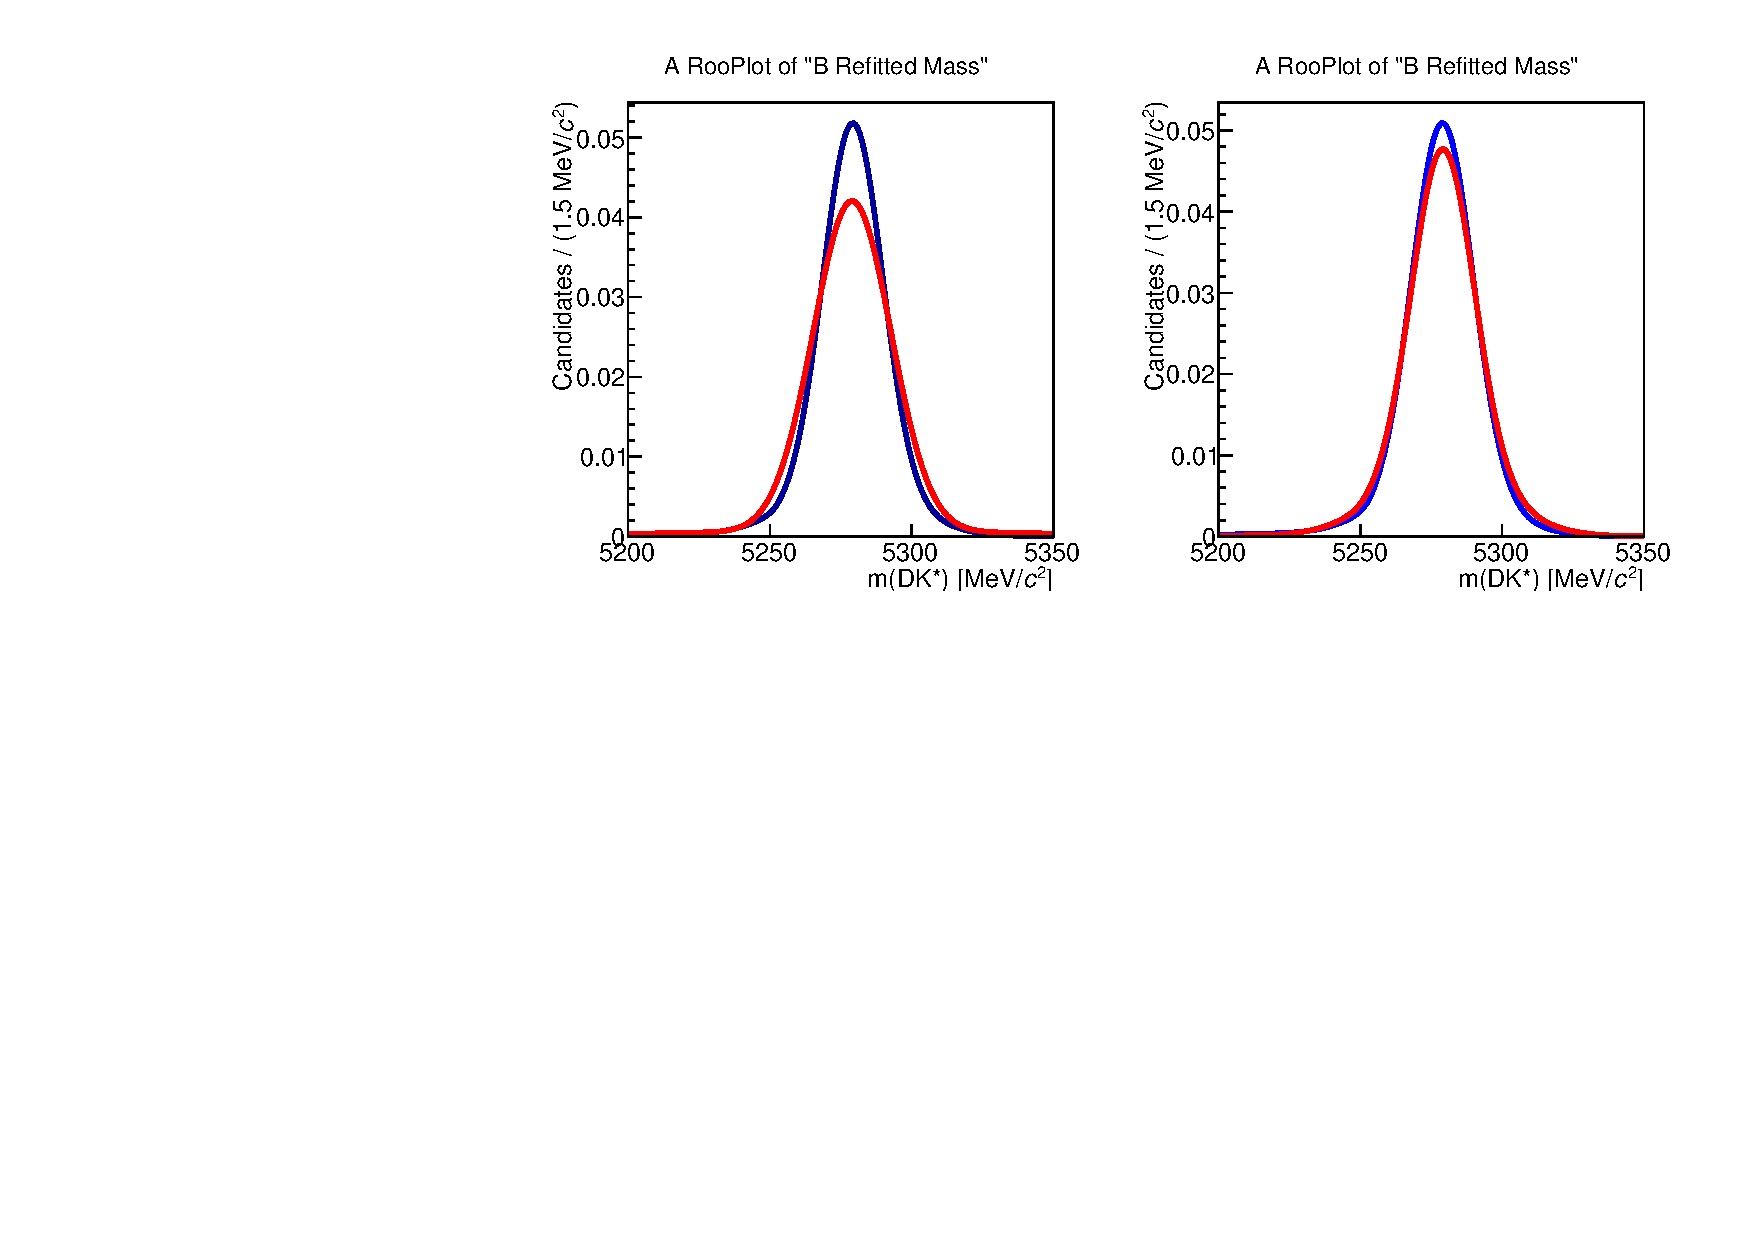
\includegraphics[width=0.7\linewidth]{figures/fitComponents/signalMC_run1_KPivsKPiPiPi.pdf}
\put(-270,110) {(a)}
\put(-120,110) {(b)}
\caption{Comparison of Run 1 signal fit functions for $K\pi$ (blue) and $K\pi\pi\pi$ (red) for (a) LL candidates and (b) DD candidates}
\label{signalfitcomparisonRun1}
\end{figure}

\begin{table}
\centering
\begin{tabular}{ccccc}
\hline
& \multicolumn{2}{c}{$K\pi$} & \multicolumn{2}{c}{$K\pi\pi\pi$} \\
& data & MC & data & MC \\
\hline
LL & $5279.3 \pm 0.6$ & $5279.12 \pm 0.15$ & $5279.6 \pm 0.9$ & $5279.62 \pm 0.12$ \\
DD & $5279.3 \pm 0.4$ & $5279.30 \pm 0.09$ & $5279.3 \pm 0.6$ & $5279.50 \pm 0.19$ \\
\hline
\end{tabular}
\caption{Fitted mean of the signal shape for $K\pi$ and $K\pi\pi\pi$. Data and MC results are found to be consistent.}
\label{signalmean}
\end{table}

\begin{figure}[!h]
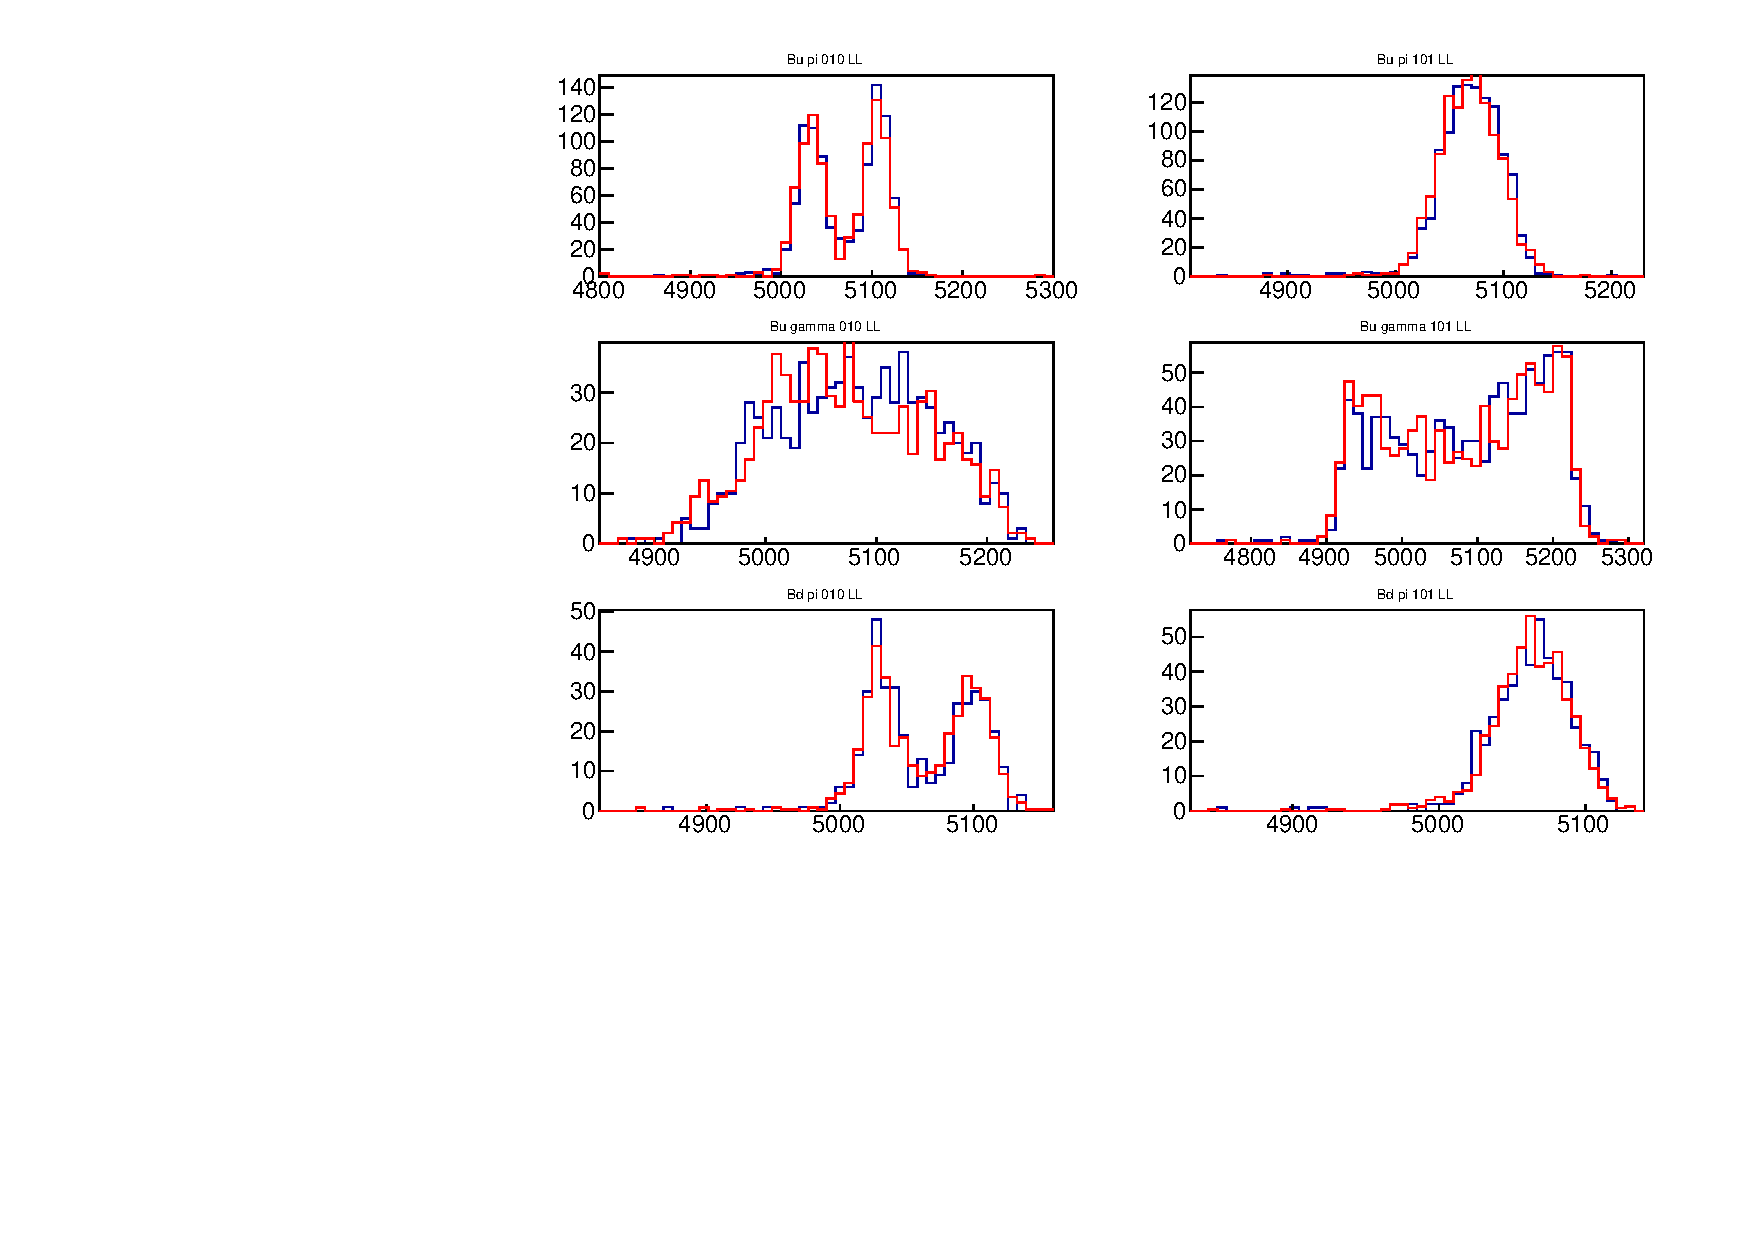
\includegraphics[width=\linewidth]{figures/compareMC/run1vsrun2MC_partreco_LL.pdf}
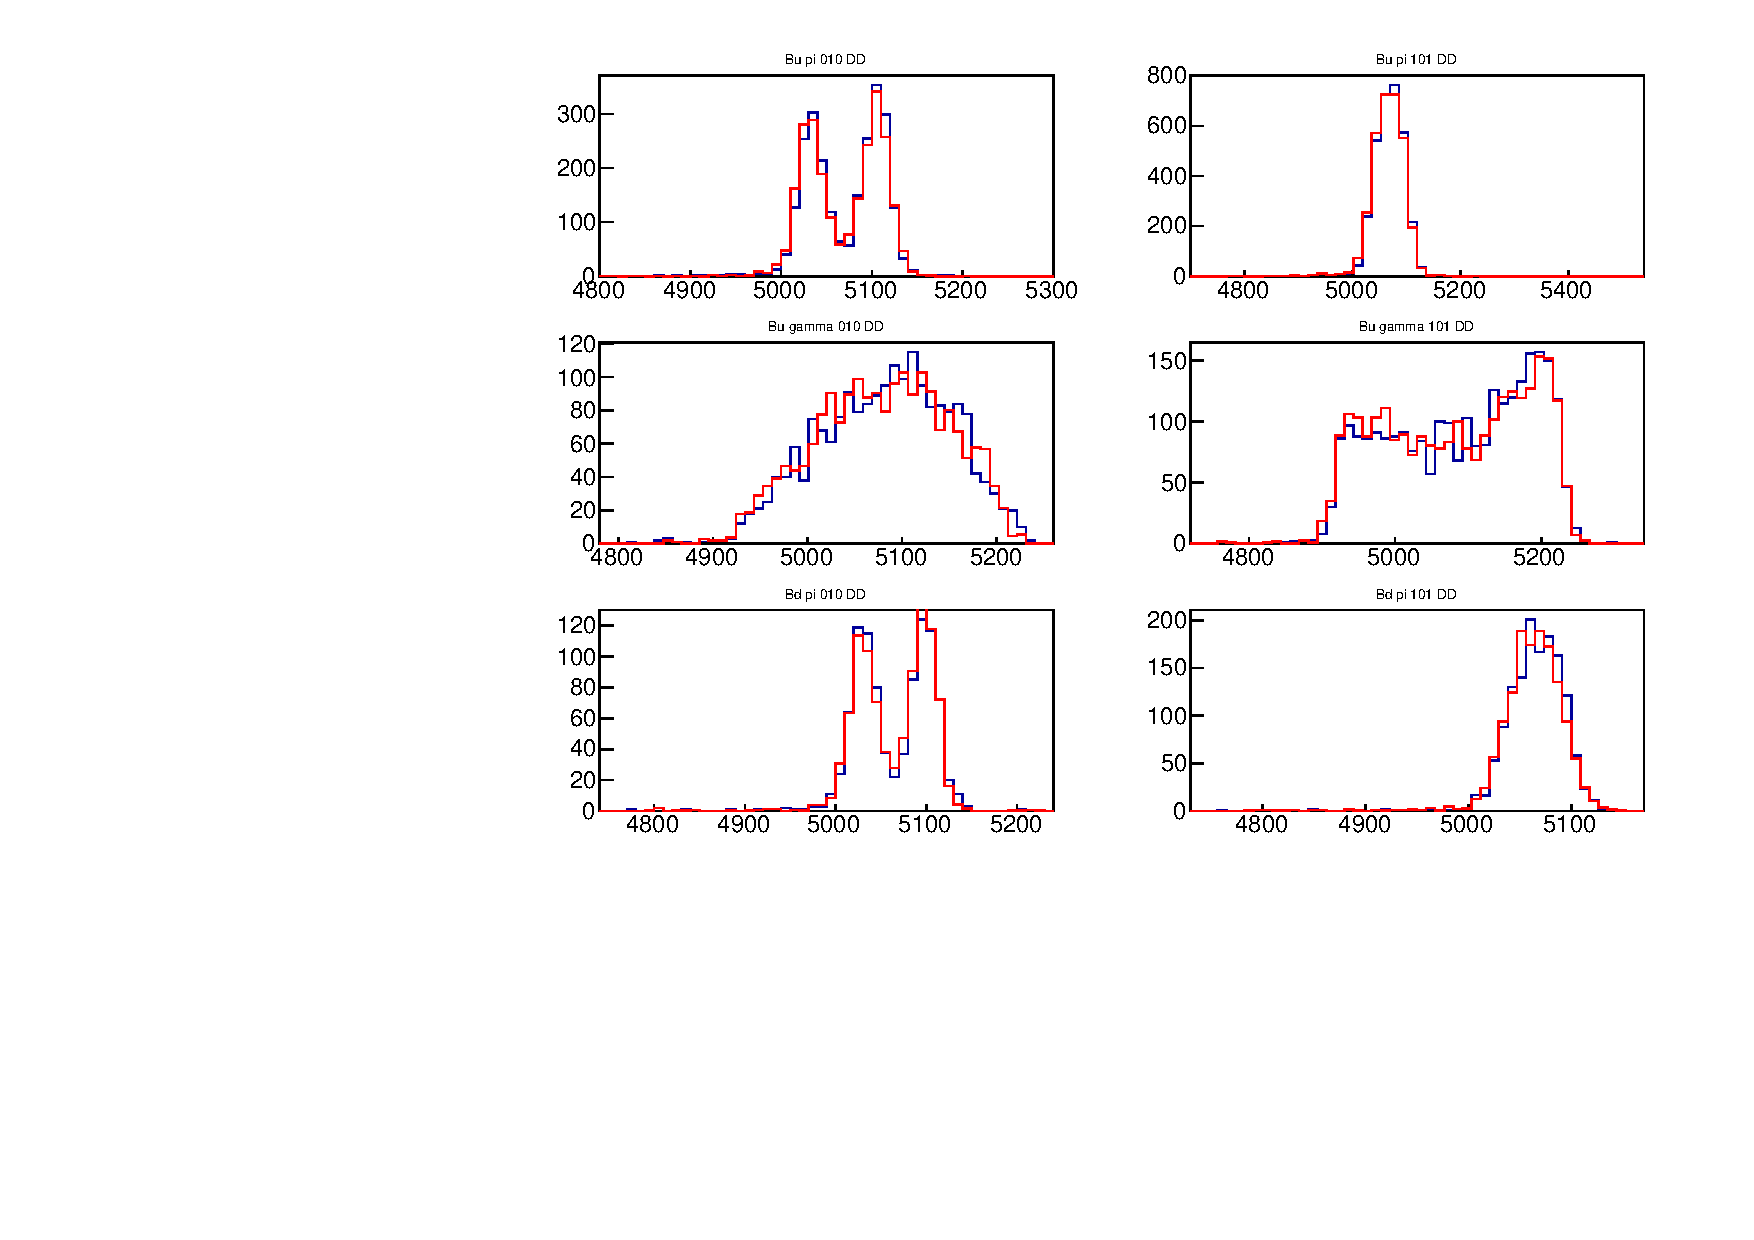
\includegraphics[width=\linewidth]{figures/compareMC/run1vsrun2MC_partreco_DD.pdf}
\caption{Comparison of partially reconstructed MC between Run 1 (blue) and 2015 (red). The different shapes correspond to different \Dstar\Kstar modes, descibed in Section \ref{sec:massfit:partreco}}
\label{parterecofits}
\end{figure}


\section{PID efficiencies}
\label{sec:mc:pid}

In this analysis the selection for the various D decays modes \decay{\D}{\kaon\pi, \kaon\kaon, \pi\pi, \pi\kaon} is almost identical apart for the particle identification requirements. Therefore it is very important to apply an efficient PID selection.

As described in Section \ref{sec:selection:pid}, the PID requirements are $DLLK < 4$ for the pion from the \Kstarm and $DLLK > 2$ and $DLLK < -2$ for the \D daughters when applied to kaons and pions respectively. The efficiencies for the various selection are determined using the {\tt PIDCalib} package~\cite{PIDCalib}. The uncertainties in the PID efficiencies are systematic and come from:

\begin{itemize}
\item The use of finite samples of \Dstar calibration tracks
\item The use of finite signal track samples
\item The {\tt PIDCalib} procedure
\end{itemize}

The PID efficiencies for $K\pi$ $KK$ and $\pi\pi$ are listed in Tables \ref{pideffkpi}, \ref{pideffkk} and \ref{pideffpipi} respectively. Similarly the PID efficienies for $K\pi\pi\pi$ and $\pi\pi\pi\pi$ are listed in Tables \ref{pideffkpipipi} and \ref{pideffpipipipi}. These PID efficiencies are used in the \CP fit as described in Equation \ref{effcorrectionglw}. The PID efficiencies are combined separately for Run 1 and Run 2 according to the efficiency corrected yields in each of the samples. 

Another input to the fit is the efficiency of the double misID veto, which is required as a correction to the ADS observables, as in Equation \ref{effcorrectionads}. The veto efficiency is sensitive to changes in the $p$ and $p_T$ of the \Dz, therefore the application of the PID selection will affect the efficiency of the veto. The signal MC samples (separated by year and magnet polarity) were reweighted to account for the effects of the PID selection, using the {\tt PIDCalib} package. The efficiency of the veto was then calculated for each of the samples and subsequently combined; the results are shown in Table \ref{vetoefficiencies}. The veto efficiencies were also calculated from data by comparing the yield in the $K\pi$ favoured mode before and after applying the veto; the results are shown in Table \ref{vetoefficienciesdata}. The veto efficiencies from data and MC are consistent with each other. Veto efficiencies calculated from data are used in the \CP fit for both two and four-body modes, given in Tables \ref{vetoefficienciesdata} and \ref{vetoefficienciesdatak3pi}.

\begin{table}[h]
\centering
\begin{tabular}{c|cc|cc}
\hline
& \multicolumn{2}{c}{LL} & \multicolumn{2}{c}{DD} \\
& MagDown & MagUp & MagDown & MagUp \\
\hline
2011 & $73.3 \pm 0.2$ & $74.3 \pm 0.2$ & $74.2 \pm 0.2$ & $74.3 \pm 0.2$ \\
2012 & $73.8 \pm 0.2$ & $72.8 \pm 0.2$ & $74.9 \pm 0.2$ & $74.8 \pm 0.2$ \\
2015 & $80.8 \pm 0.2$ & $80.9 \pm 0.2$ & $82.0 \pm 0.2$ & $82.0 \pm 0.2$ \\
2016 & $80.6 \pm 0.2$ & $81.9 \pm 0.2$ & $81.8 \pm 0.2$ & $82.4 \pm 0.2$ \\
\hline
Run 1 combined & \multicolumn{2}{c}{$73.4 \pm 0.2$} & \multicolumn{2}{c}{$74.7 \pm 0.2$} \\
Run 2 combined & \multicolumn{2}{c}{$81.1 \pm 0.2$} & \multicolumn{2}{c}{$82.1 \pm 0.2$} \\
\hline
\end{tabular}
\caption{PID efficiencies for \decay{\Dz}{\Km\pip} in 2011, 2012, 2015 and 2016 data for both magnet polarities. These numbers are given as percentages}
\label{pideffkpi}
\end{table}

\begin{table}[h]
\centering
\begin{tabular}{c|cc|cc}
\hline
& \multicolumn{2}{c}{LL} & \multicolumn{2}{c}{DD} \\
& MagDown & MagUp & MagDown & MagUp \\
\hline
2011 & $81.6 \pm 0.2$ & $81.7 \pm 0.2$ & $82.5 \pm 0.2$ & $82.8 \pm 0.2$ \\
2012 & $81.1 \pm 0.2$ & $81.0 \pm 0.2$ & $83.4 \pm 0.2$ & $81.6 \pm 0.2$ \\
2015 & $85.1 \pm 0.2$ & $84.4 \pm 0.2$ & $86.2 \pm 0.2$ & $85.4 \pm 0.2$ \\
2016 & $84.3 \pm 0.2$ & $84.4 \pm 0.2$ & $85.0 \pm 0.2$ & $85.4 \pm 0.2$ \\
\hline
Run 1 combined & \multicolumn{2}{c}{$81.2 \pm 0.2$} & \multicolumn{2}{c}{$82.5 \pm 0.2$} \\
Run 2 combined & \multicolumn{2}{c}{$84.4 \pm 0.2$} & \multicolumn{2}{c}{$85.3 \pm 0.2$} \\
\hline
\end{tabular}
\caption{PID efficiencies for \decay{\Dz}{\Kp\Km} in 2011, 2012, 2015 and 2016 data for both magnet polarities. These numbers are given as percentages}
\label{pideffkk}
\end{table}

\begin{table}[h]
\centering
\begin{tabular}{c|cc|cc}
\hline
& \multicolumn{2}{c}{LL} & \multicolumn{2}{c}{DD} \\
& MagDown & MagUp & MagDown & MagUp \\
\hline
2011 & $65.2 \pm 0.2$ & $64.9 \pm 0.2$ & $66.3 \pm 0.2$ & $66.9 \pm 0.2$ \\
2012 & $68.0 \pm 0.2$ & $67.2 \pm 0.2$ & $68.8 \pm 0.2$ & $67.4 \pm 0.2$ \\
2015 & $78.4 \pm 0.2$ & $77.0 \pm 0.2$ & $79.6 \pm 0.2$ & $78.7 \pm 0.2$ \\
2016 & $76.6 \pm 0.2$ & $79.2 \pm 0.2$ & $78.1 \pm 0.2$ & $79.7 \pm 0.2$ \\
\hline
Run 1 combined & \multicolumn{2}{c}{$67.0 \pm 0.2$} & \multicolumn{2}{c}{$67.6 \pm 0.2$} \\
Run 2 combined & \multicolumn{2}{c}{$77.9 \pm 0.2$} & \multicolumn{2}{c}{$79.0 \pm 0.2$} \\
\hline
\end{tabular}
\caption{PID efficiencies for \decay{\Dz}{\pip\pim} in 2011, 2012, 2015 and 2016 data for both magnet polarities. These numbers are given as percentages}
\label{pideffpipi}
\end{table}

\begin{table}[h]
\centering
\begin{tabular}{c|cc|cc}
\hline
& \multicolumn{2}{c}{LL} & \multicolumn{2}{c}{DD} \\
& MagDown & MagUp & MagDown & MagUp \\
\hline
2011 & - & - & - & - \\
2012 & $64.3 \pm 0.2$ & $61.7 \pm 0.2$ & $64.7 \pm 0.2$ & $62.6 \pm 0.2$ \\
2015 & $79.0 \pm 0.2$ & $77.6 \pm 0.2$ & $80.5 \pm 0.2$ & $79.9 \pm 0.2$ \\
2016 & $77.7 \pm 0.2$ & $79.1 \pm 0.2$ & $79.1 \pm 0.2$ & $80.4 \pm 0.2$ \\
\hline
Run 1 combined & \multicolumn{2}{c}{$63.0 \pm 0.2$} & \multicolumn{2}{c}{$63.6 \pm 0.2$} \\
Run 2 combined & \multicolumn{2}{c}{$78.4 \pm 0.2$} & \multicolumn{2}{c}{$79.8 \pm 0.2$} \\
\hline
\end{tabular}
\caption{PID efficiencies for \decay{\Dz}{\Km\pip\pim\pip} in 2012, 2015 and 2016 data for both magnet polarities. These numbers are given as percentages}
\label{pideffkpipipi}
\end{table}

\begin{table}[h]
\centering
\begin{tabular}{c|cc|cc}
\hline
& \multicolumn{2}{c}{LL} & \multicolumn{2}{c}{DD} \\
& MagDown & MagUp & MagDown & MagUp \\
\hline
2011 & - & - & - & - \\
2012 & & & & \\
2015 &  &  &  &  \\
2016 & & & & \\
\hline
Run 1 combined & \multicolumn{2}{c}{} & \multicolumn{2}{c}{} \\
Run 2 combined & \multicolumn{2}{c}{} & \multicolumn{2}{c}{} \\
\hline
\end{tabular}
\caption{PID efficiencies for \decay{\Dz}{\pip\pim\pip\pim} in 2012, 2015 and 2016 data for both magnet polarities. These numbers are given as percentages {\color{red} Will be updated when the MC is available}}
\label{pideffpipipipi}
\end{table}

\begin{table}
\centering
\begin{tabular}{c|cc|cc}
\hline
& \multicolumn{2}{c}{LL} & \multicolumn{2}{c}{DD} \\
& MagDown & MagUp & MagDown & MagUp \\
\hline
2011 & $93.2 \pm 1.2$ & $93.3 \pm 1.2$ & $92.6 \pm 0.8$ & $93.4 \pm 0.8$ \\
2012 & $94.0 \pm 1.3$ & $91.5 \pm 1.4$ & $93.7 \pm 0.8$ & $92.3 \pm 0.8$ \\
2015 & $93.7 \pm 1.1$ & $92.6 \pm 1.2$ & $91.9 \pm 0.8$ & $92.8 \pm 0.7$ \\
2016 & $93.1 \pm 0.7$ & $92.5 \pm 0.7$ & $92.2 \pm 0.4$ & $93.4 \pm 0.4$ \\
\hline
Run 1 combined & \multicolumn{2}{c}{$92.9 \pm 0.8$} & \multicolumn{2}{c}{$93.0 \pm 0.4$} \\
Run 2 combined & \multicolumn{2}{c}{$92.9 \pm 0.4$} & \multicolumn{2}{c}{$92.7 \pm 0.3$} \\
\hline
\end{tabular}
\caption{Veto efficiencies for 2 body mode taken from 2011, 2012 and 2015 MC for LL and DD candidates. These numbers are given as percentages}
\label{vetoefficiencies}
\end{table}

\begin{table}
\centering
\begin{tabular}{ccc}
\hline
& LL & DD \\
\hline
Run 1 & $90.5 \pm 0.9$ & $91.9 \pm 0.5$ \\
Run 2 & $91.5 \pm 0.7$ & $91.7 \pm 0.4$ \\
\hline
\end{tabular}
\caption{Veto efficiencies for 2 body mode calculated from data. These numbers are given as percentages}
\label{vetoefficienciesdata}
\end{table}

\begin{table}
\centering
\begin{tabular}{ccc}
\hline
& LL & DD \\
\hline
Run 1 & $89.5 \pm 0.5$ & $88.2 \pm 0.3$ \\
Run 2 & $91.6 \pm 0.3$ & $90.6 \pm 0.2$ \\
\hline
\end{tabular}
\caption{Veto efficiencies for 4 body mode calculated from data. These numbers are given as percentages}
\label{vetoefficienciesdatak3pi}
\end{table}

Tables \ref{pideffkpi}, \ref{pideffkk}, \ref{pideffpipi} and \ref{pideffkpipipi} show that the PID efficiency in Run 2 is higher than Run 1 for the PID selection used in this analysis. In order to check that the PID selection for Run 1 is suitable to be applied to Run 2 the misID efficiency (efficiency of a $K\pi$ candidate passing the $\pi K$ PID selection) was investigated; the results are shown in Table \ref{misideff} and \ref{misideff4body}. For the 2-body mode, both the PID efficiency and misID efficiency is improved in Run 2 compared to Run 1 so the same PID selection can be applied to both datasets. For the 4-body mode the misID efficiency is slightly worse in Run 2 compared to Run 1. A low misID rate is required to reduce the crossfeed background discussed in Section \ref{sec:backgrounds:crossfeed}, which reports a negligible level of this crossfeed background in both Run 1 and Run 2, therefore the misID rate is already sufficiently low and  sothe PID selection does not need to be tightened for Run 2.

\begin{table}[h]
\centering
\begin{tabular}{c|cc|cc}
\hline
& \multicolumn{2}{c}{LL} & \multicolumn{2}{c}{DD} \\
& MagDown & MagUp & MagDown & MagUp \\
\hline
2011 & $0.143$ & $0.139$ & $0.143$ & $0.157$ \\
2012 & $0.150$ & $0.177$ & $0.131$ & $0.151$ \\
2015 & $0.098$ & $0.117$ & $0.099$ & $0.112$ \\
2016 & $0.119$ & $0.108$ & $0.111$ & $0.098$ \\
\hline
Run 1 combined & \multicolumn{2}{c}{$0.158$} & \multicolumn{2}{c}{$0.144$} \\
Run 2 combined & \multicolumn{2}{c}{$0.112$} & \multicolumn{2}{c}{$0.104$} \\
\hline
\end{tabular}
\caption{MisID efficiencies for \decay{\Dz}{\Km\pip} to \decay{\Dz}{\Kp\pim}. The numbers are given as percentages. Errors in these values are O(0.001), but the exact uncertainties are not important as the values are not used in the mass fit}
\label{misideff}
\end{table}

\begin{table}[h]
\centering
\begin{tabular}{c|cc|cc}
\hline
& \multicolumn{2}{c}{LL} & \multicolumn{2}{c}{DD} \\
& MagDown & MagUp & MagDown & MagUp \\
\hline
2011 & - & - & - & - \\
2012 & $0.084$ & $0.093$ & $0.073$ & $0.095$ \\
2015 & $0.093$ & $0.146$ & $0.109$ & $0.106$ \\
2016 & $0.127$ & $0.105$ & $0.122$ & $0.088$ \\
\hline
Run 1 combined & \multicolumn{2}{c}{$0.089$} & \multicolumn{2}{c}{$0.084$} \\
Run 2 combined & \multicolumn{2}{c}{$0.115$} & \multicolumn{2}{c}{$0.106$} \\
\hline
\end{tabular}
\caption{MisID efficiencies for \decay{\Dz}{\Km\pip\pim\pip} to \decay{\Dz}{\Kp\pim\pip\pim}. The numbers are given as percentages. Errors in these values are O(0.001), but the exact uncertainties are not important as the values are not used in the mass fit}
\label{misideff4body}
\end{table}

\section{Efficiency inputs in \CP fit}

The \CP fit, described in Section \ref{sec:cpfit} uses efficiency calculations from MC, as detailed in Section \ref{sec:mc:efficiencies}. Signal efficiencies, BDT efficiencies, PID efficiencies and double misID veto efficiency are estimated from MC for LL and DD and used separately in the \CP fit. Table \ref{fitinputs} summarises the values used in the \CP fit. 

\begin{table}
\centering
\begin{tabular}{c|cc|cc}
\hline
& \multicolumn{2}{c}{Run 1} & \multicolumn{2}{c}{Run 2} \\
& LL & DD & LL & DD \\
\hline
$BF(\decay{\Dz}{\Km\pip})$ & \multicolumn{4}{c}{$0.0393 \pm 0.0004$} \\
$BF(\decay{\Dz}{\Kp\Km})$ & \multicolumn{4}{c}{$0.00401 \pm 0.00007$} \\
$BF(\decay{\Dz}{\pip\pim})$ & \multicolumn{4}{c}{$0.001421 \pm 0.000025$} \\
$\epsilon_{sel}(K\pi)$ & $0.0939 \pm 0.0011$ & $0.2519 \pm 0.0018$ & $0.1266 \pm 0.0011$ & $0.3155 \pm 0.0017$ \\
$\epsilon_{sel}(KK)$ & $0.0919 \pm 0.0011$ & $0.2450 \pm 0.0018$ & $0.1189 \pm 0.0010$ & $0.2923 \pm 0.0016$ \\
$\epsilon_{sel}(\pi\pi)$ & $0.1015 \pm 0.0012$ & $0.2584 \pm 0.0018$ & $0.1292 \pm 0.0011$ & $0.3309 \pm 0.0017$ \\
$\epsilon_{pid}(K\pi)$ & $0.734 \pm 0.002$ & $0.747 \pm 0.002$ & $0.811 \pm 0.002$ & $0.821 \pm 0.002$ \\
$\epsilon_{pid}(KK)$ & $0.812 \pm 0.002$ & $0.825 \pm 0.002$ & $0.844 \pm 0.002$ & $0.853 \pm 0.002$ \\
$\epsilon_{pid}(\pi\pi)$ & $0.670 \pm 0.002$ & $0.676 \pm 0.002$ & $0.779 \pm 0.002$ & $0.790 \pm 0.002$ \\
$\epsilon_{bdt}(K\pi)$ & $0.947 \pm 0.005$ & $0.896 \pm 0.004$ & $0.949 \pm 0.003$ & $0.907 \pm 0.002$ \\
$\epsilon_{bdt}(\pi K)$ & $0.947 \pm 0.005$ & $0.802 \pm 0.005$ & $0.949 \pm 0.003$ & $0.826 \pm 0.003$ \\
$\epsilon_{veto}(\pi K)$ & $0.905 \pm 0.009$ & $0.919 \pm 0.005$ & $0.915 \pm 0.007$ & $0.917 \pm 0.004$ \\
$\epsilon_{sel}(K\pi\pi\pi)$ & $0.0288 \pm 0.0006$ & $0.0816 \pm 0.0020$ & $0.0484 \pm 0.0004$ & $0.1229 \pm 0.0007$ \\
$\epsilon_{sel}(\pi\pi\pi\pi)$ & $0.0311 \pm 0.0006$ & $0.0837 \pm 0.0020$ & $0.0494 \pm 0.0004$ & $0.1289 \pm 0.0007$ \\
$\epsilon_{pid}(K\pi\pi\pi)$ & $0.630 \pm 0.002$ & $0.636 \pm 0.002$ & $0.784 \pm 0.002$ & $0.798 \pm 0.002$ \\
$\epsilon_{pid}(\pi\pi\pi\pi)$ & $0.575 \pm 0.002$ & $0.576 \pm 0.002$ & $0.753 \pm 0.002$ & $0.768 \pm 0.002$ \\
$\epsilon_{bdt}(K\pi\pi\pi)$ & $0.938 \pm 0.010$ & $0.903 \pm 0.007$ & $0.952 \pm 0.003$ & $0.928 \pm 0.002$ \\
$\epsilon_{bdt}(\pi K\pi\pi)$ & $0.938 \pm 0.010$ & $0.838 \pm 0.009$ & $0.952 \pm 0.003$ & $0.870 \pm 0.003$ \\
$\epsilon_{veto}(\pi K \pi\pi)$ & $0.895 \pm 0.005$ & $0.882 \pm 0.003$ & $0.916 \pm 0.003$ & $0.906 \pm 0.002$ \\
\hline
\end{tabular}
\caption{Table of branching fractions and efficiencies used in the \CP fit. Branching ratios are taken from the PDG~\cite{PDG2014}. All these values are fixed inputs and systematics are assigned based on the uncertainties, as detailed in Section \ref{sec:systematics}. The Run 2 uncertainties are inflated compared to 2015 assuming 2016 MC efficiencies have the same central value as 2015 but with twice the uncertainty. {\color{red} Efficiencies for $\pi\pi\pi\pi$ mode are place holders (close to the correct values) until the MC is available}}
\label{fitinputs}
\end{table}


\clearpage
